\subsection{Clean-Data Baseline}

On noiseless waveforms the hybrid model achieves perfect classification
on all splits, including a held-out set of unseen deviation types.
This establishes that the architecture can learn the deviation
structure when noise is absent.

\subsection{Synthetic Noise: SNR Sweep}

Using synthetic aLIGO-PSD noise with $\beta \in [0.3, 1.0]$ we sweep
the SNR from $5$ to $50$. Table~\ref{tab:synth_snr} shows the results.
The detection threshold in synthetic noise is approximately
$\text{SNR} \approx 20$. Figure~\ref{fig:detection_vs_snr} shows the
corresponding accuracy-versus-SNR curve.

\begin{table}[h]
\centering
\caption{Synthetic-noise SNR sweep, amplitude $\beta \in [0.3, 1.0]$.}
\label{tab:synth_snr}
\begin{tabular}{lccc}
\toprule
SNR bin & val acc & test\_seen & test\_unseen \\
\midrule
30--50 & 1.000 & 1.000 & 1.000 \\
15--20 & 0.771 & 0.755 & 0.846 \\
10--15 & 0.750 & 0.735 & 0.686 \\
8--10  & 0.688 & 0.776 & 0.551 \\
5--8   & 0.667 & 0.776 & 0.538 \\
\bottomrule
\end{tabular}
\end{table}

\begin{figure}[h]
\centering
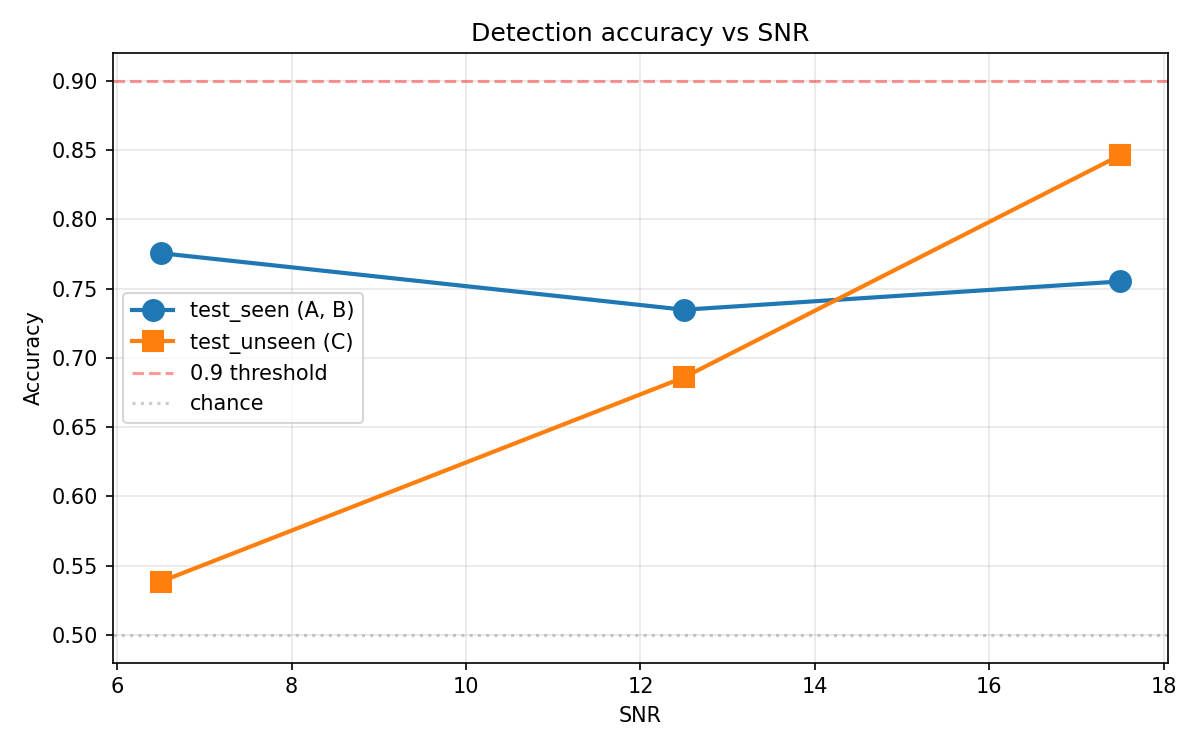
\includegraphics[width=0.7\linewidth]{figures/detection_vs_snr.png}
\caption{Detection accuracy versus SNR for synthetic aLIGO noise,
amplitude modulation with $\beta \in [0.3, 1.0]$.}
\label{fig:detection_vs_snr}
\end{figure}

\subsection{Real LIGO Noise: SNR Sweep}

Using real H1 strain and $\beta \in [5, 20]$ we obtain
Table~\ref{tab:real_snr}. For strong deviations, detection is robust
across the entire SNR range tested.

\begin{table}[h]
\centering
\caption{Real LIGO noise SNR sweep, amplitude $\beta \in [5, 20]$.}
\label{tab:real_snr}
\begin{tabular}{lccc}
\toprule
SNR bin & val acc & test\_seen & test\_unseen \\
\midrule
30--50 & 1.000 & 1.000 & 0.974 \\
20--30 & 1.000 & 1.000 & 0.987 \\
15--20 & 1.000 & 1.000 & 0.968 \\
10--15 & 0.979 & 0.980 & 0.968 \\
5--10  & 0.979 & 1.000 & 0.968 \\
\bottomrule
\end{tabular}
\end{table}

\subsection{Threshold in $\beta$ at Fixed SNR}

At $\text{SNR} = 10$--$15$ with real noise, we sweep $\beta$ from
$0.1$ to $20$. Table~\ref{tab:beta_sweep} shows the transition from
chance performance at $\beta \leq 0.2$ to reliable detection at
$\beta \geq 0.5$. The detection threshold is $\beta \approx 0.4$ for
the injected $30 + 25 M_\odot$ configuration.

\begin{table}[h]
\centering
\caption{$\beta$ sweep at SNR $10$--$15$, real LIGO noise.}
\label{tab:beta_sweep}
\begin{tabular}{lcc}
\toprule
$\beta$ range & test\_seen & test\_unseen \\
\midrule
0.1--0.5  & 0.735 & 0.500 \\
0.3--0.5  & 0.918 & 0.891 \\
0.5--2.0  & 0.898 & 0.930 \\
2.0--5.0  & 0.939 & 0.923 \\
5.0--20.0 & 0.980 & 0.968 \\
\bottomrule
\end{tabular}
\end{table}

\subsection{Deviation-Type Comparison}

Table~\ref{tab:dev_types} compares amplitude, phase, and frequency
modulation at matched $\beta$ ranges. All three deviation types are
detected with high accuracy. Figure~\ref{fig:dev_types} summarizes
the comparison.

\begin{table}[h]
\centering
\caption{Deviation-type comparison, SNR $10$--$15$, real noise, N = 200.}
\label{tab:dev_types}
\begin{tabular}{lcc}
\toprule
Deviation & test\_seen & test\_unseen \\
\midrule
Amplitude, $\beta \in [0.5, 2.0]$ & 0.898 & 0.930 \\
Phase,     $\beta \in [0.5, 2.0]$ & 0.878 & 0.930 \\
Frequency, $\beta \in [5, 25]$    & 0.878 & 0.885 \\
\bottomrule
\end{tabular}
\end{table}

\begin{figure}[h]
\centering
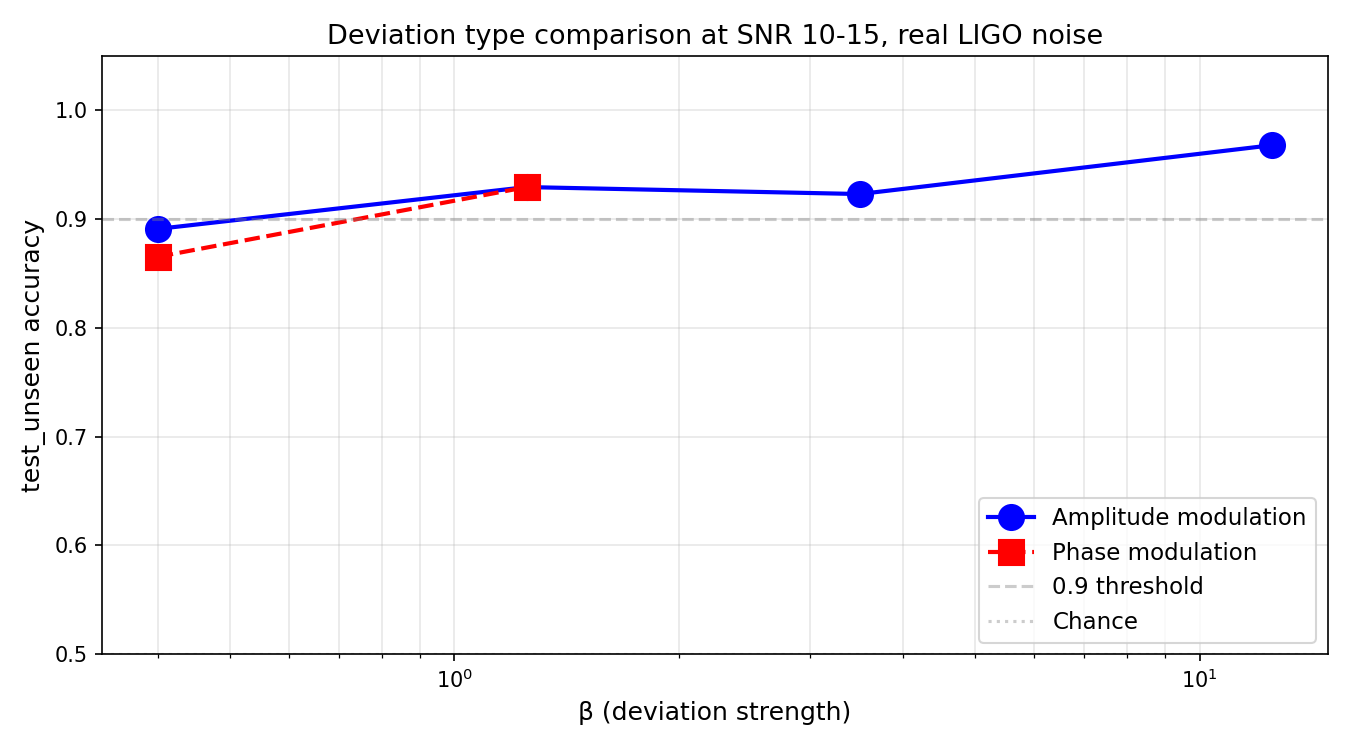
\includegraphics[width=0.7\linewidth]{figures/deviation_type_comparison.png}
\caption{Accuracy on unseen deviation types for amplitude and phase
modulation at matched $\beta$ ranges.}
\label{fig:dev_types}
\end{figure}

\begin{figure}[h]
\centering
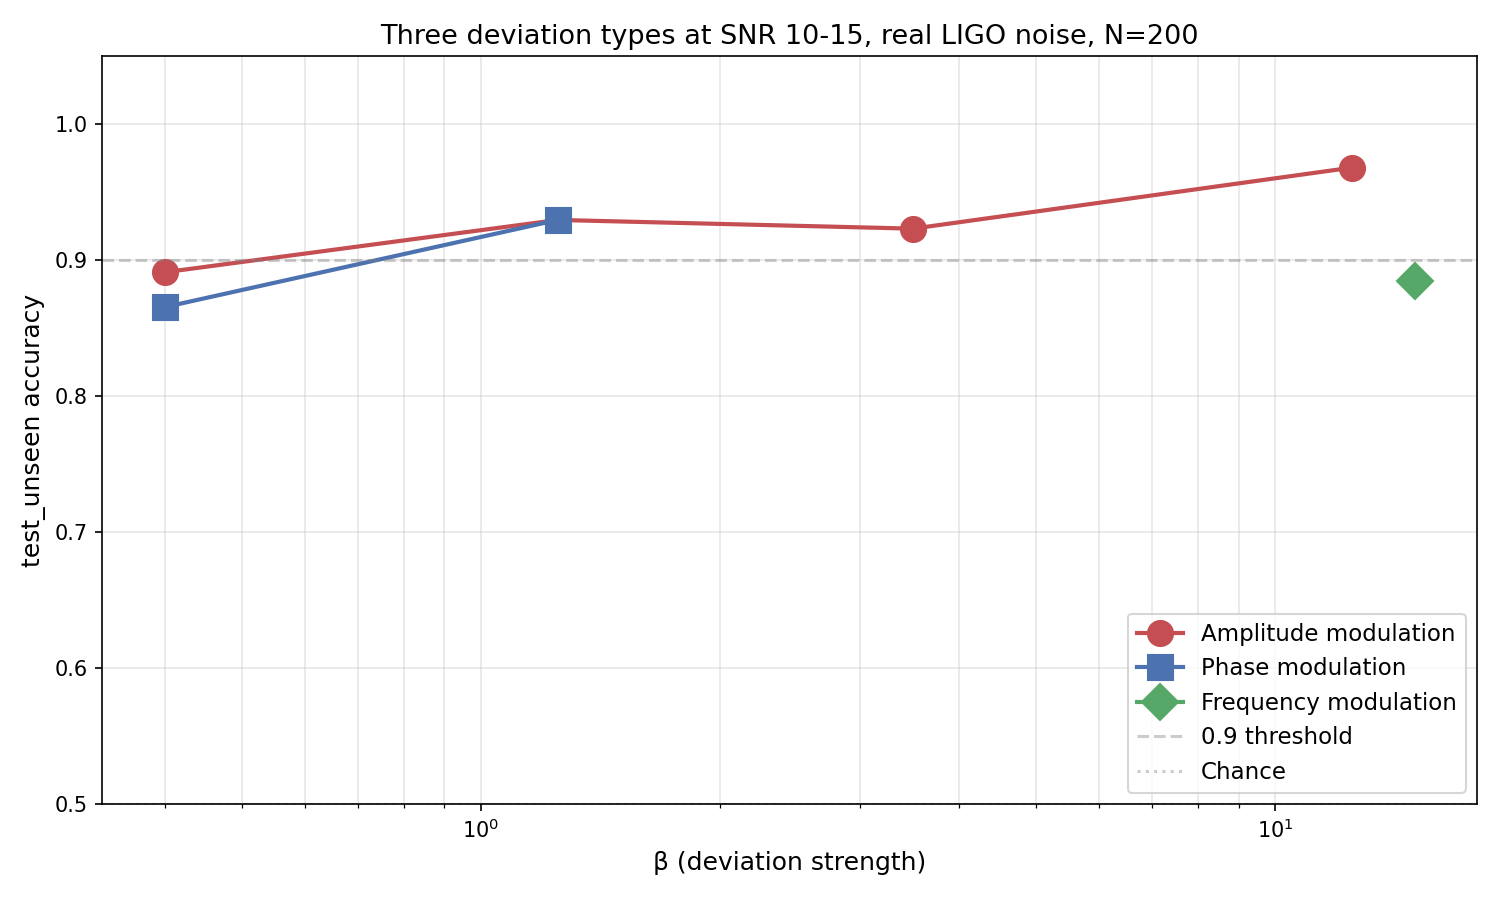
\includegraphics[width=0.7\linewidth]{figures/three_deviation_types.png}
\caption{Detection accuracy for all three deviation families in real
LIGO noise, SNR $10$--$15$.}
\label{fig:three_dev}
\end{figure}

\subsection{Mass-Ratio Generalization}

Four mass configurations spanning $q = 1$ to $q = 10$ give test-unseen
accuracies between $0.891$ and $0.930$, with a standard deviation of
$1.7$ percentage points. Table~\ref{tab:mass_ratio} lists the values,
and Figure~\ref{fig:mass_ratio} shows the distribution.

\begin{table}[h]
\centering
\caption{Mass-ratio generalization, amplitude $\beta \in [0.5, 2.0]$,
SNR $10$--$15$.}
\label{tab:mass_ratio}
\begin{tabular}{lcc}
\toprule
$(m_1, m_2)$ [$M_\odot$] & $q$ & test\_unseen \\
\midrule
$(30, 30)$ & 1.0 & 0.904 \\
$(30, 25)$ & 1.2 & 0.930 \\
$(40, 10)$ & 4.0 & 0.891 \\
$(50, 5)$  & 10.0 & 0.917 \\
\bottomrule
\end{tabular}
\end{table}

\begin{figure}[h]
\centering
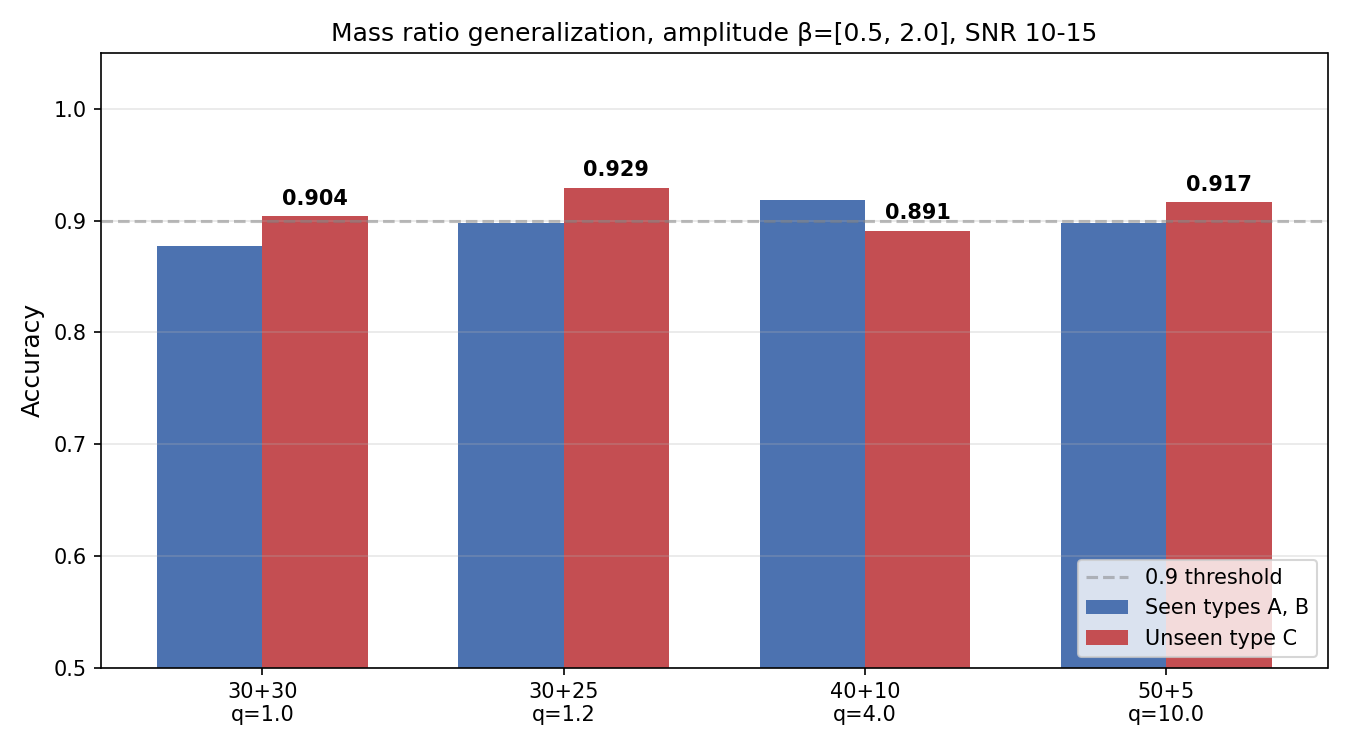
\includegraphics[width=0.7\linewidth]{figures/mass_ratio_generalization.png}
\caption{Mass-ratio generalization of the hybrid classifier in real
LIGO noise at SNR $10$--$15$.}
\label{fig:mass_ratio}
\end{figure}

\subsection{GW150914 Amplitude Detectability Curve}

Using the real GW150914 strain as a template and sweeping $\beta$
from $0.01$ to $20$, we obtain the detectability curve in
Figure~\ref{fig:detectability_curve} and Table~\ref{tab:beta_curve}.
Accuracy rises smoothly from chance at $\beta \leq 0.2$ to perfect
classification at $\beta \geq 0.5$. The transition is centered at
$\beta \approx 0.25$.

\begin{table}[h]
\centering
\caption{GW150914 amplitude-controlled detectability curve, SNR = 20.}
\label{tab:beta_curve}
\begin{tabular}{lccc}
\toprule
$\beta$ range & val acc & test\_seen & test\_unseen \\
\midrule
$0.01$--$0.2$ & 0.717 & 0.717 & 0.517 \\
$0.2$--$0.3$  & 0.850 & 0.850 & 0.750 \\
$0.3$--$0.4$  & 0.950 & 0.950 & 0.900 \\
$0.4$--$0.5$  & 0.983 & 0.983 & 0.967 \\
$0.5$--$1.0$  & 1.000 & 1.000 & 1.000 \\
$5$--$20$     & 1.000 & 1.000 & 1.000 \\
\bottomrule
\end{tabular}
\end{table}

\begin{figure}[h]
\centering
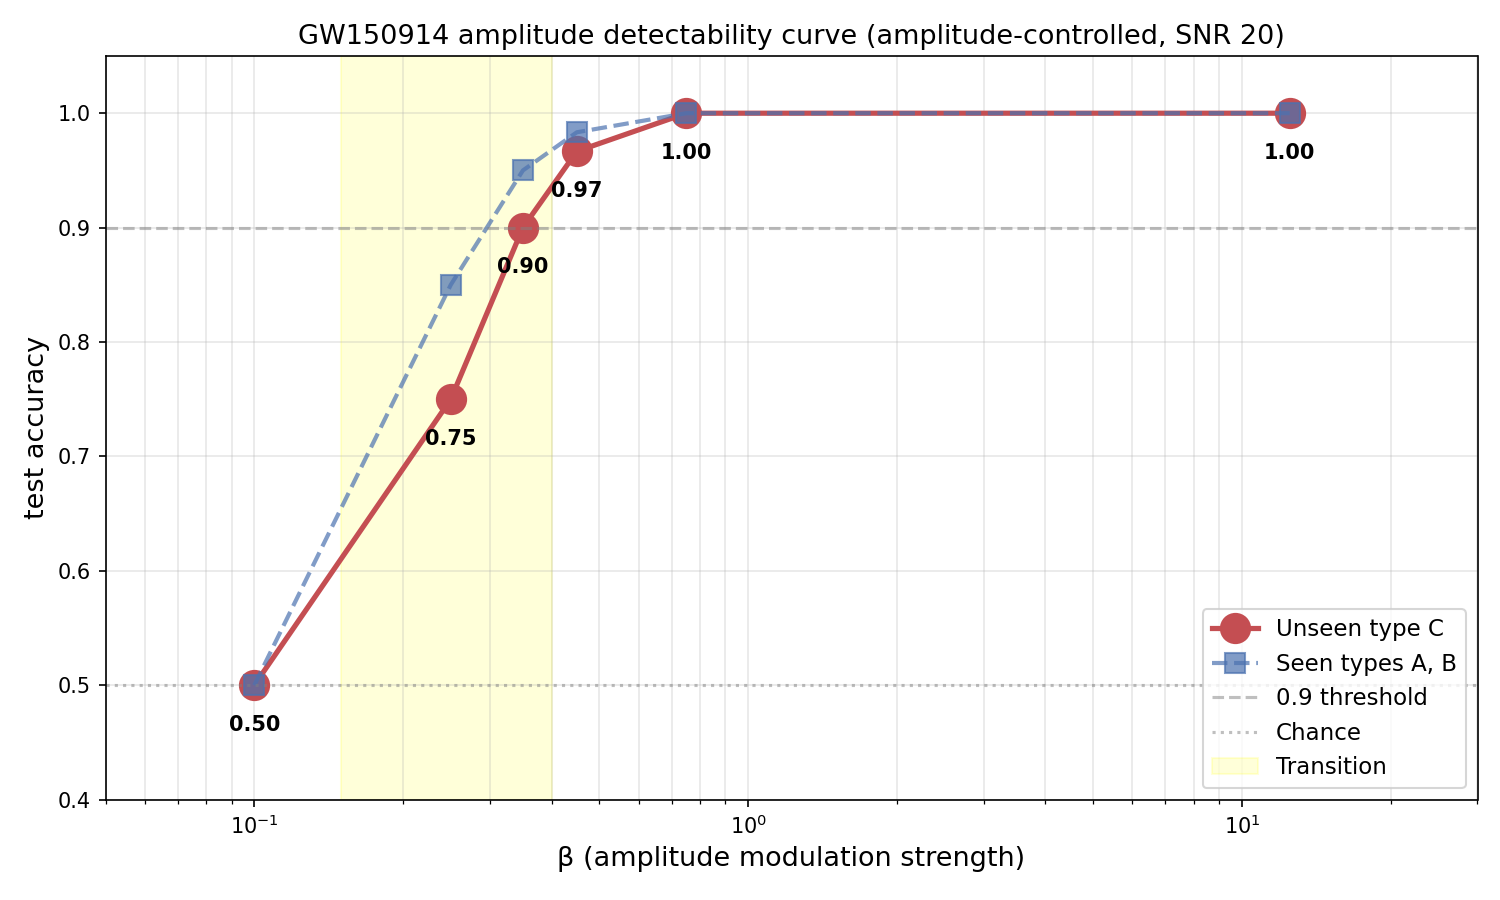
\includegraphics[width=0.75\linewidth]{figures/beta_detectability_curve.png}
\caption{Amplitude detectability curve for the GW150914 template.
Unseen-type-C accuracy rises smoothly from chance
($\beta \leq 0.2$) to perfect classification
($\beta \geq 0.5$). The transition is centered at
$\beta \approx 0.25$.}
\label{fig:detectability_curve}
\end{figure}

\subsection{Feature-Importance Analysis}

A random forest trained on nine statistical features achieves $100\%$
validation accuracy at $\beta \in [0.5, 2.0]$. The most important
features are mean absolute amplitude ($0.284$), the top-1000 mean
($0.279$) and the $99$th percentile of $|x|$ ($0.263$). Standard
deviation and RMS are useless, with importances $0.0000$ and $0.0001$
respectively. The classifier therefore relies on tail statistics that
capture the shape of the modulation rather than its overall scale.

\subsection{Negative Result at Small $\beta$}

For $\beta \in [0.01, 0.2]$, the classifier fails: training accuracy
$0.586$, validation accuracy $0.717$, and test-unseen accuracy $0.517$
(chance). The loss remains at the chance level $\ln 2 \approx 0.693$
throughout training, indicating that the model cannot find a
discriminative feature.
